%%%%%%%%%%%%%%%%%%%%%%%%%%%%%%%%%%%%%%%%%
% Journal Article
% LaTeX Template
% Version 1.4 (15/5/16)
%
% This template has been downloaded from:
% http://www.LaTeXTemplates.com
%
% Original author:
% Frits Wenneker (http://www.howtotex.com) with extensive modifications by
% Vel (vel@LaTeXTemplates.com)
%
% License:
% CC BY-NC-SA 3.0 (http://creativecommons.org/licenses/by-nc-sa/3.0/)
%
%%%%%%%%%%%%%%%%%%%%%%%%%%%%%%%%%%%%%%%%%

%----------------------------------------------------------------------------------------
%	PACKAGES AND OTHER DOCUMENT CONFIGURATIONS
%----------------------------------------------------------------------------------------

\documentclass[twoside,twocolumn]{article}
  
  \usepackage{blindtext} % Package to generate dummy text throughout this template 
  
  \usepackage{graphicx} %Include graphics
  \graphicspath{{./img/}}

  \usepackage{amsmath} % Use math notation
  \newcommand{\realset}{\mathbb{R}} % Include real set char
  \usepackage{ upgreek }

  \usepackage[sc]{mathpazo} % Use the Palatino font
  \usepackage[T1]{fontenc} % Use 8-bit encoding that has 256 glyphs
  \linespread{1.05} % Line spacing - Palatino needs more space between lines
  \usepackage{microtype} % Slightly tweak font spacing for aesthetics
  
  \usepackage[spanish]{babel}
  \selectlanguage{spanish}
  \usepackage[utf8]{inputenc} % Include utf-8 character renderization
  
  \usepackage[hmarginratio=1:1,top=32mm,columnsep=20pt]{geometry} % Document margins
  \usepackage[hang, small,labelfont=bf,up,textfont=it,up]{caption} % Custom captions under/above floats in tables or figures
  \usepackage{booktabs} % Horizontal rules in tables
  
  \usepackage{lettrine} % The lettrine is the first enlarged letter at the beginning of the text
  
  \usepackage{enumitem} % Customized lists
  \setlist[itemize]{noitemsep} % Make itemize lists more compact
  
  \usepackage{abstract} % Allows abstract customization
  \renewcommand{\abstractnamefont}{\normalfont\bfseries} % Set the "Abstract" text to bold
  \renewcommand{\abstracttextfont}{\normalfont\small\itshape} % Set the abstract itself to small italic text
  
  \usepackage{titlesec} % Allows customization of titles
  % \renewcommand\thesection{\Roman{section}} % Roman numerals for the sections
  % \renewcommand\thesubsection{\roman{subsection}} % roman numerals for subsections
  % \titleformat{\section}[block]{\large\scshape\centering}{\thesection.}{1em}{} % Change the look of the section titles
  % \titleformat{\subsection}[block]{\large}{\thesubsection.}{1em}{} % Change the look of the section titles
  
  \usepackage{fancyhdr} % Headers and footers
  \pagestyle{fancy} % All pages have headers and footers
  \fancyhead{} % Blank out the default header
  \fancyfoot{} % Blank out the default footer
  \fancyhead[LE]{Introducción al Aprendizaje Automático} % Custom header text
  \fancyhead[RO]{David Omar Flores Chávez} % Custom header text
  \fancyfoot[RO,LE]{\thepage} % Custom footer text

  \usepackage{titling} % Customizing the title section
  
  \usepackage{hyperref} % For hyperlinks in the PDF
  
  %----------------------------------------------------------------------------------------
  %	TITLE SECTION
  %----------------------------------------------------------------------------------------
  
  \setlength{\droptitle}{-4\baselineskip} % Move the title up
  
  \pretitle{\begin{center}\Huge} % Article title formatting
  \posttitle{\end{center}} % Article title closing formatting
  
  \title{Introducción al Aprendizaje Automático
    \large \\[2\baselineskip]
    Intuición, Algoritmos y Mejores Prácticas
    \\[2\baselineskip]
  } % Article title
  
  \author{
      \textsc{David Omar Flores Chávez} \\[1ex] % Your name
      \normalsize Escuela Superior de Cómputo \\ % Your institution
      \normalsize {davidomarfch@gmail.com}\\[2\baselineskip] % Your email address
      % \and % Uncomment if 2 authors are required, duplicate these 4 lines if more
      % \textsc{Héctor Aguilar Hernández} \\[1ex] % Second author's name
      % \normalsize Escuela Superior de Cómputo \\ % Second author's institution
      % \normalsize {hectoraldairah@gmail.com} % Second author's email address
  }
  
  \date{\today} % Leave empty to omit a date
  
  \renewcommand{\maketitlehookd}{%
  \begin{abstract}
      \noindent Este artículo pretende resaltar la importancia
      de la intuición de los algoritmos más utlizados en el aprendizaje automático.
      También se proporcionará una pequeña guía de visualización de datos para
      realizar las exploraciones iniciales en cada problema.
      El objetivo, es que más allá de saber cómo implementarlos, el lector sepa elegir
      qué algoritmo es el apropiado para un conjunto de datos en particular, ahorrando
      tiempo y recursos técnicos y humanos.
  \end{abstract}
  }
  
  %----------------------------------------------------------------------------------------
  
  \begin{document}
  
  % Print the title
  \maketitle
  %----------------------------------------------------------------------------------------
  %	ARTICLE CONTENTS
  %----------------------------------------------------------------------------------------
  
  \section{Introducción}
  
    % \lettrine[nindent=0em,lines=3]{E} 
    El Aprendizaje Automático, 
    Aprendizaje de Máquinas o \textit{Machine Learning} es una rama
    de la inteligencia artificial que pretende otorgar a las computadoras
    la \textbf{capacidad de aprender}.

    El término fue acuñado en 1959 por el informático Arthur M. Samuel, y lo
    definió como \textit{«el campo de estudio que le otorga a las computadoras
    la habilidad de aprender, sin ser programadas de manera explícita.»} \cite{Samuel:1959:SML:1661923.1661924}

    Tom Mitchell, en el año de 1997, propone una definición más formal para el
    término: \textit{«Una computadora aprende de la experiencia E, con respecto a
    una tarea T, y una medida de rendimiento P, si su rendimiento en la tarea T,
    siendo medido por P, mejora con la experiencia E»} \cite{Mitchell1997}

  %------------------------------------------------
  
  \section{Tipos de Algoritmos}
  
      Los algoritmos de aprendizaje pueden clasificarse en tres
      categorías principales, tomando como criterio las 
      características de los datos con que se entrenan:

      \begin{itemize}
        \item Aprendizaje supervisado
        \item Aprendizaje no-supervisado
        \item Aprendizaje por refuerzo
      \end{itemize}

      \subsection{Aprendizaje Supervisado} 
        Permite inferir información a partir de un conjunto de
        datos etiquetados\footnote{Grupo de muestras cuyas características
        han sido etiquetadas para crear datos más significativos.}.

        Cada muestra consiste de

        \begin{enumerate}[label=(\alph*)]
          \item \textbf{una entrada}, y
          \item \textbf{una salida esperada.}
        \end{enumerate}
        
        Este tipo de aprendizaje analiza los datos de entrenamiento,
        aprende de ellos, y produce una \textbf{función} que puede usarse
        para \textit{mapear} nuevas muestras.

        Ejemplos de posibles aplicaciones de estos algoritmos, pueden ser:

        \begin{itemize}
          \item Aprendiendo del tamaño, velocidad de crecimiento (entrada),
                y el tipo (salida) de miles de tumores, predecir si un
                tumor diferente será benigno o maligno.
          \item Aprendiendo del tamaño, estilo arquitectónico, 
                número de baños (entrada), y costo (salida)
                de miles de casas, predecir un nuevo costo de una casa diferente.
        \end{itemize}

      \subsection{Aprendizaje No Supervisado}
        Permite descubrir -tanto si existe, como si no-, alguna estructura
        oculta dentro de un conjunto de datos.

        Dado que la característica principal de este tipo de aprendizaje
        es la utilización de datos no etiquetados, es imposible conocer
        la validez de la estructura descubierta por el algoritmo.

        Ejemplos de posibles aplicaciones de estos algoritmos, pueden ser:
        
        \begin{itemize}
          \item Analizando una base de datos de miles de clientes,
                poder generar distintos segmentos de mercado,
                y describir las cualidades de cada uno.
          \item Analizando una enorme cantidad de fotos, separarlas
                todas, utilizando como criterio de separación la cara
                de las personas que aparecen en las fotos.
        \end{itemize}

    \section{Regresión}
        
        Los problemas de regresión son útiles en la predicción de 
        \textbf{valores reales}.

        Comencemos con un ejemplo motivador para la predicción del costo 
        de viviendas.
        
        Usaremos un conjunto de datos ficticio que contiene
        \begin{enumerate}[label=(\alph*)]
          \item el tamaño de una vivienda en pies cuadrados, y
          \item el precio de la vivienda en miles de dólares
        \end{enumerate}

        Si intentamos visualizar la distribución de los datos, tendremos la
        siguiente gráfica:

        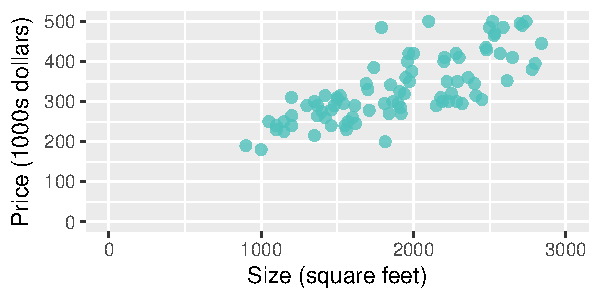
\includegraphics[width=\columnwidth, page = 1]{housePrices.pdf}

        Ahora, imaginemos que tenemos una vivienda de 1250 $ft^2$ y
        nos interesa tener una idea de cuál es el precio que podría
        alcanzar en el mercado.

        \includegraphics[width=\columnwidth, page = 2]{housePrices.pdf}

        Para hacerlo, podemos intentar \textbf{ajustar un modelo} a la gráfica,
        y usarlo para hacer nuestras predicciones.

        Ajustando una línea recta, podemos estimar que una vivienda de
        1250 $ft^2$, tiene un costo de \$ USD 250, 000.

        \includegraphics[width=\columnwidth, page = 3]{housePrices.pdf}
        
        Este es un ejemplo de \textbf{aprendizaje supervisado}: cada
        \textit{evento} de nuestro conjunto de datos cuenta con la 
        \textit{salida esperada}: el precio de cada vivienda.

        \subsection{Nomenclatura y notación}
          Más formalmente, en el aprendizaje supervisado, tenemos un conjunto
          de datos llamado \textbf{conjunto de entrenamiento}.

          El conjunto de entrenamiento contiene $m$ ejemplos $(\upchi, y)$, donde
          $\upchi$ es una variable de entrada, e $y$ una variable de salida.

          Ambos valores son vectores de dimensión $m$.

          \[
            \upchi
            ,
            y \in \realset^{m}
          \]

          Para referirnos a un elemento $i$ dentro del conjunto, utilizamos la notación
          $\upchi^{(i)}$ e $y^{(i)}$ siempre que $1 \leq i \leq m$.

          Es importante que al usar esta notación, se entienda que no se
          trata de exponenciación.
        
          \[
            \upchi^{(i)} \ne \upchi^i
          \]

          Cuando la variable de entrada tiene \textbf{más de una característica},
          $\upchi$ es una matriz de $m \times n$ dimensiones,
         
          \[
            \upchi \in \realset^{m \times n}
          \]

          donde $n$ es el número de características de cada entrada.

          Nótese que si $n = 1 \implies \upchi \in \realset ^ {m \times 1}$, por lo que 
          $\upchi$ es un vector de dimensión $m$.

          Para referirnos a una característica $j$ específica, utilizamos la notación
          $\upchi_{j}$ siempre que $1 \leq j \leq n$.

          Apliquemos la notación mencionada para tratar de explorar el conjunto de datos
          de la siguiente tabla.

          \begin{table}[h]

            \centering
            \caption{Conjunto de entrenamiento.}
            \label{tabla:m_datos}

            \resizebox{\columnwidth}{!}{%
              \begin{tabular}{@{}rrrrr@{}}

                \toprule
                
                  \textbf{Ejemplo} &
                  \textbf{Tamaño} &
                  \textbf{N. Hab.} &
                  \textbf{N. Baños} &
                  \textbf{Costo} \\

                \midrule

                  $1$ & 1160 & 2 & 1 &  468  \\
                  $2$ & 1620 & 4 & 1.75 &  385  \\
                  $3$ & 990 & 3 & 1 &  210  \\
                  $4$ & 2753 & 3 & 2.5 &  1135  \\
                  $5$ & 1980 & 2 & 1.75 &  585  \\
                  $6$ & 1000 & 3 & 1 &  204  \\

                \bottomrule

              \end{tabular}
            }
          \end{table}
          
          Sabemos que nuestro conjunto de datos cuenta con una variable de entrada $\upchi$,
          y una variable de salida $y$.

          La variable de entrada $\upchi$ tiene las características de: 
          \begin{enumerate}
            \item área,
            \item número de habitaciones,
            \item número de baños
          \end{enumerate}

          El tamaño del conjunto es $m = 6$, y el número de características
          de $\upchi$ es $n = 3$, por lo tanto,

          \[
            \upchi \in \realset^{6 \times 3}
            ,
            y \in \realset^{6}
          \]

          Y los valores de cada variable son:

          \[
            \upchi
            =
            \begin{bmatrix}
              1160 & 2 & 1 \\
              1620 & 4 & 1.75 \\
              990 & 3 & 1 \\
              2753 & 3 & 2.5 \\
              1980 & 2 & 1.75 \\
              1000 & 3 & 1 \\ 
            \end{bmatrix}
            ,
            y
            =
            \begin{bmatrix}
              468  \\
              385  \\
              210  \\
              1135  \\
              585  \\
              204
            \end{bmatrix}
          \]

          Si queremos referirnos al tercer ejemplo, 

          \[
            (\upchi^{(3)}, y^{(3)})
            =
            (\begin{bmatrix}
              990 & 3 & 1
            \end{bmatrix},
            210)
          \]

          Si queremos referirnos a la primer característica,

          \[
            \upchi_1
            =
            \begin{bmatrix}
              1160 \\
              1620 \\
              990 \\
              2753 \\
              1980 \\
              1000
            \end{bmatrix}
          \]

          Y si queremos saber el número de baños del 5to ejemplo, 

          \[
            \upchi^{(5)}_3
            =
            1.75
          \]
%----------------------------------------------------------------------------------------
  %	REFERENCE LIST
  %----------------------------------------------------------------------------------------
  \bibliographystyle{unsrt}
  \bibliography{references}
  %----------------------------------------------------------------------------------------
  
  \end{document}
  